% ============================================================
%  Exercise 7 -- Transmission Lines
%  1-page landscape handout, 4 slide boxes per page
% ============================================================
\documentclass[a4paper,landscape,11pt]{article}
\usepackage[utf8]{inputenc}
\usepackage{graphicx}
\usepackage{amsmath}
\usepackage{geometry}
\usepackage{tikz}
\usepackage{booktabs}
\usepackage{helvet}
\usepackage{xcolor}

\renewcommand{\familydefault}{\sfdefault}

\geometry{margin=1cm}

% ---- Slide box ----
\newcommand{\slidebox}[2]{%
    \begin{tikzpicture}
        \draw[thick, draw=black!60, rounded corners=2pt] (0,0) rectangle (13.5, 8.5);
        \node[anchor=north west, inner sep=0pt, yshift=-5pt] at (0,0) {\footnotesize #1};
        \clip (0.1,0.1) rectangle (13.4,8.4);
        \node[anchor=center] at (6.75, 4.25) {
            \begin{minipage}{12.5cm}
                #2
            \end{minipage}
        };
    \end{tikzpicture}%
}

\begin{document}
\pagestyle{empty}

% ==================== PAGE 1 ====================
\noindent
\slidebox{1}{
    % Empty for reference
}
\hfill
\slidebox{2}{
    % Empty for reference
}

\vspace{0.7cm}

\noindent
\slidebox{3}{
    % Empty for reference
}
\hfill
\slidebox{4}{
    \centering
    \vspace{1.5cm}
    \Huge \textbf{Exercise 7} \\[0.6cm]
    \Large \textbf{Transmission Lines} \\[0.8cm]
    \normalsize
    \textcolor{black!70}{Distributed RC Models, Propagation Delay, \\ \& Slow-Edge Analysis}
}

\newpage

% ==================== PAGE 2 ====================
\noindent
\slidebox{5}{
    \centering
    \textbf{$\pi$-Topology: Propagation Delay vs N}\\[0.15cm]
    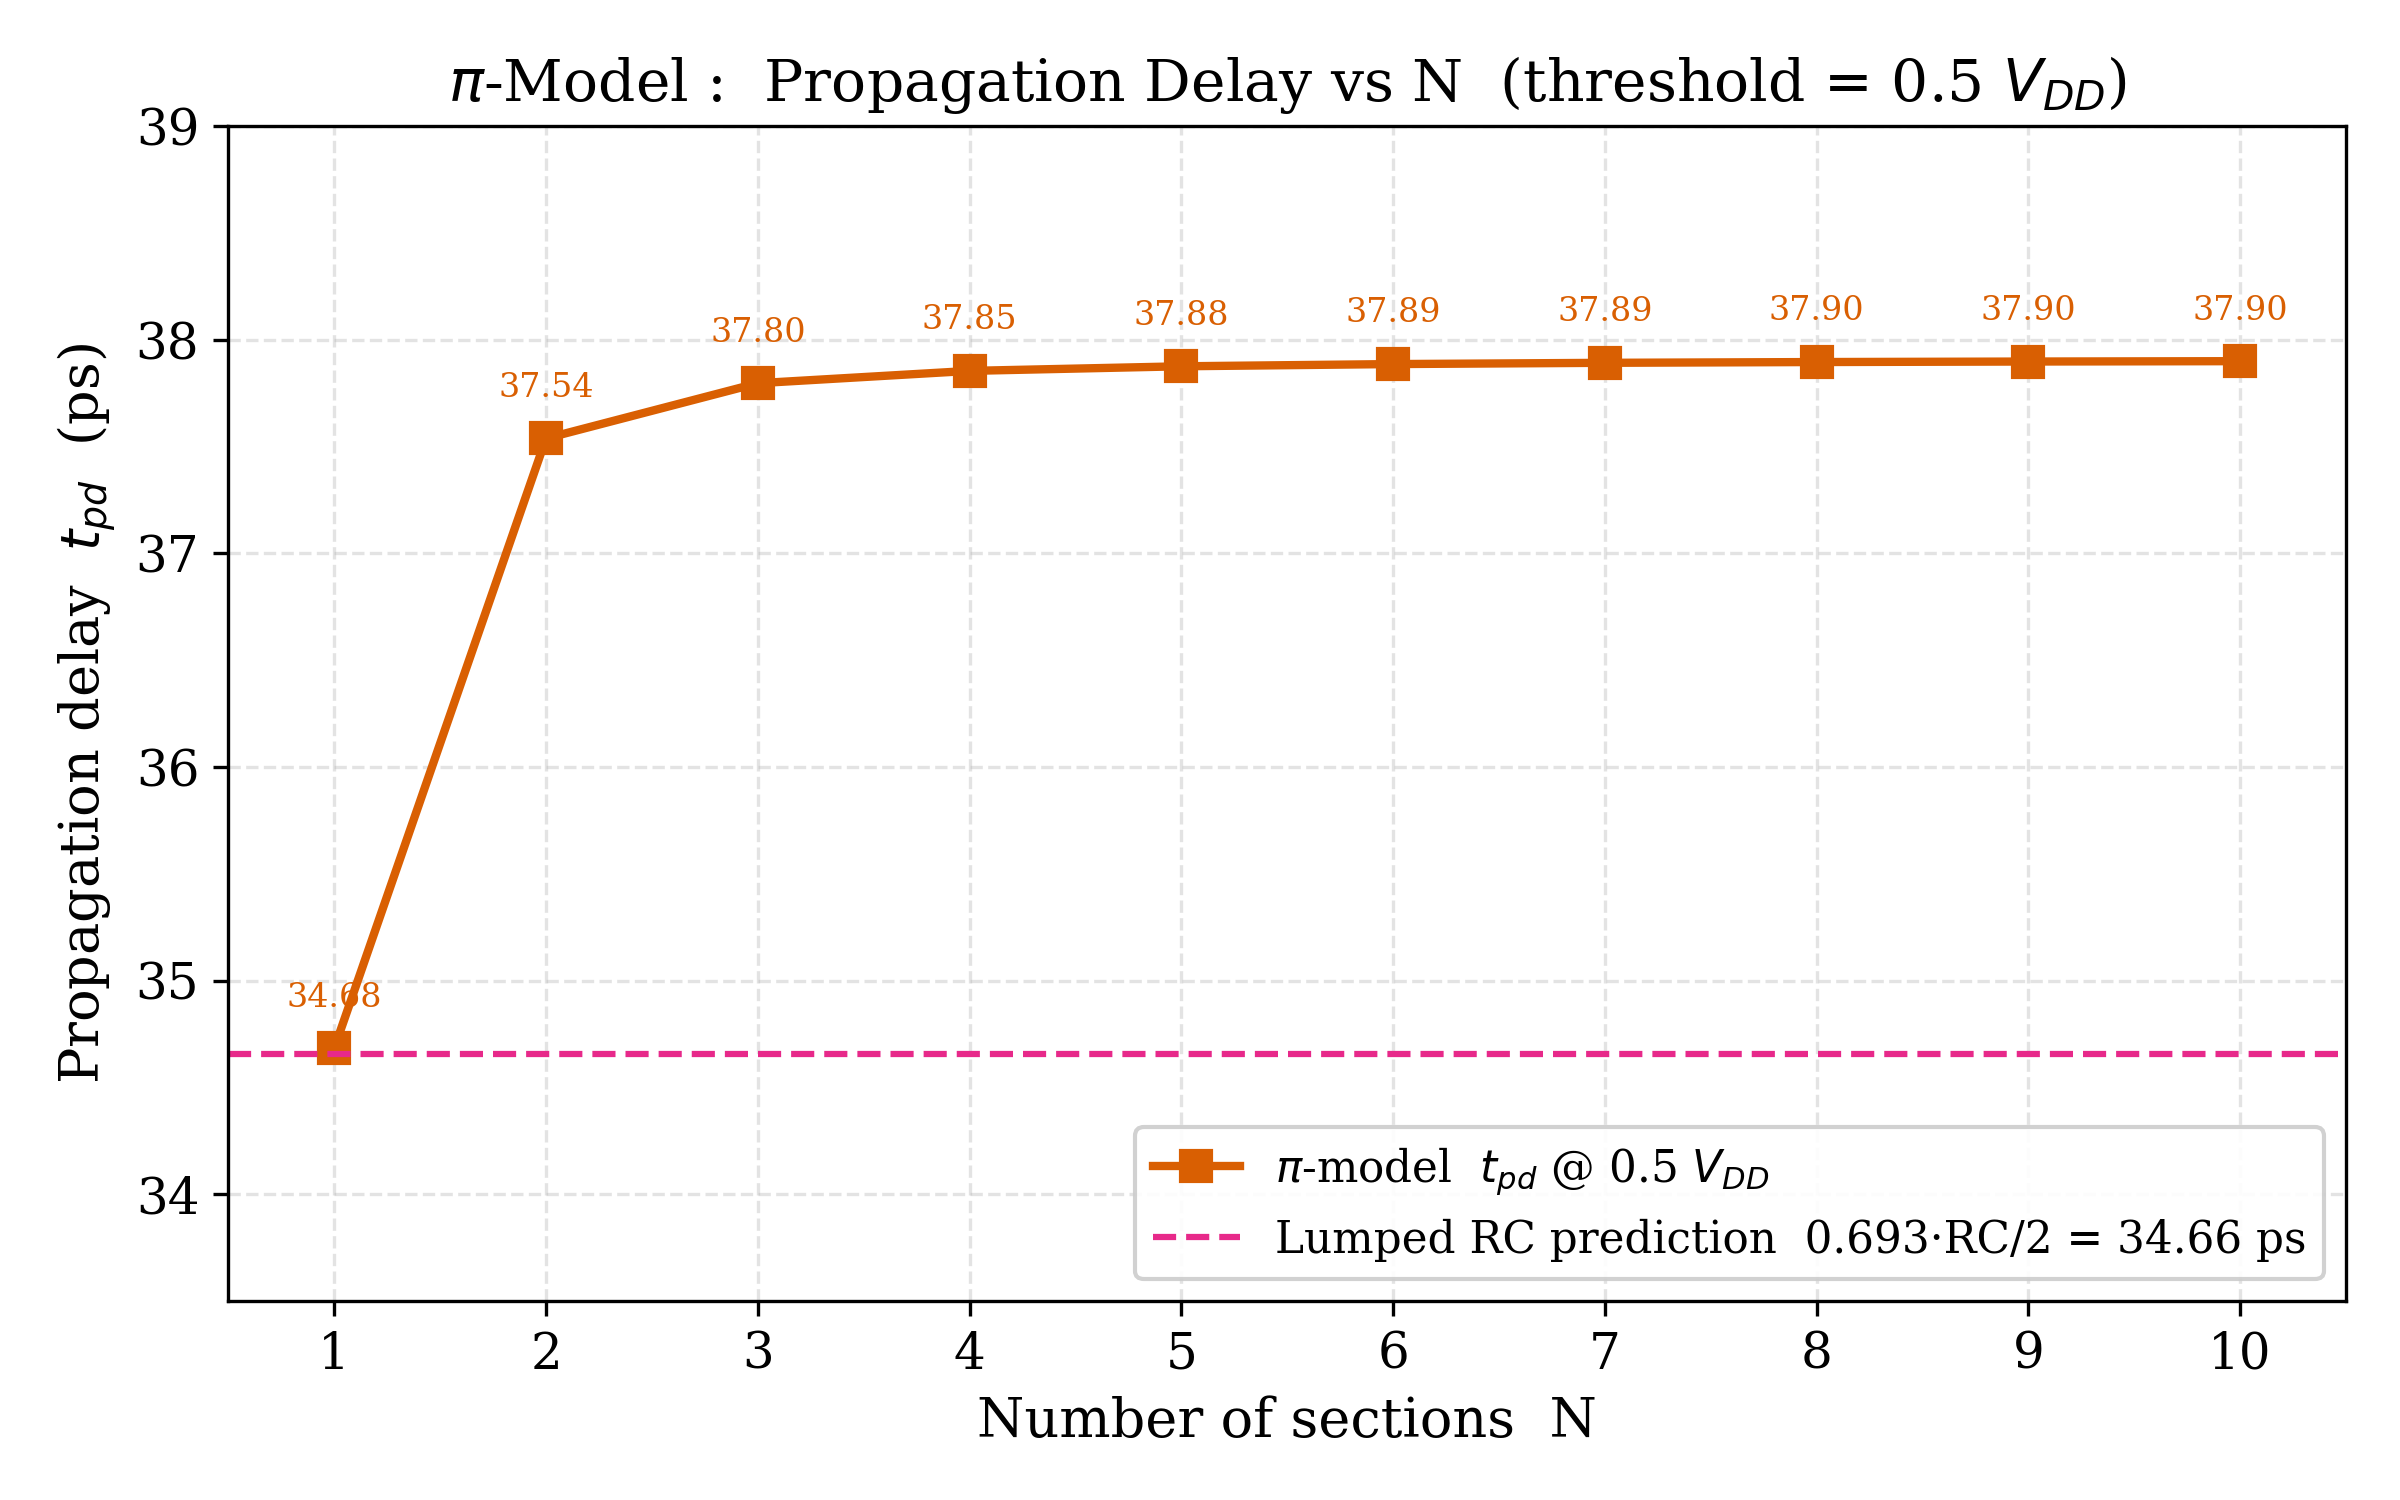
\includegraphics[width=6.1cm]{pi_topology/images/pi_tpd_vs_N_50VDD.png}\hfill
    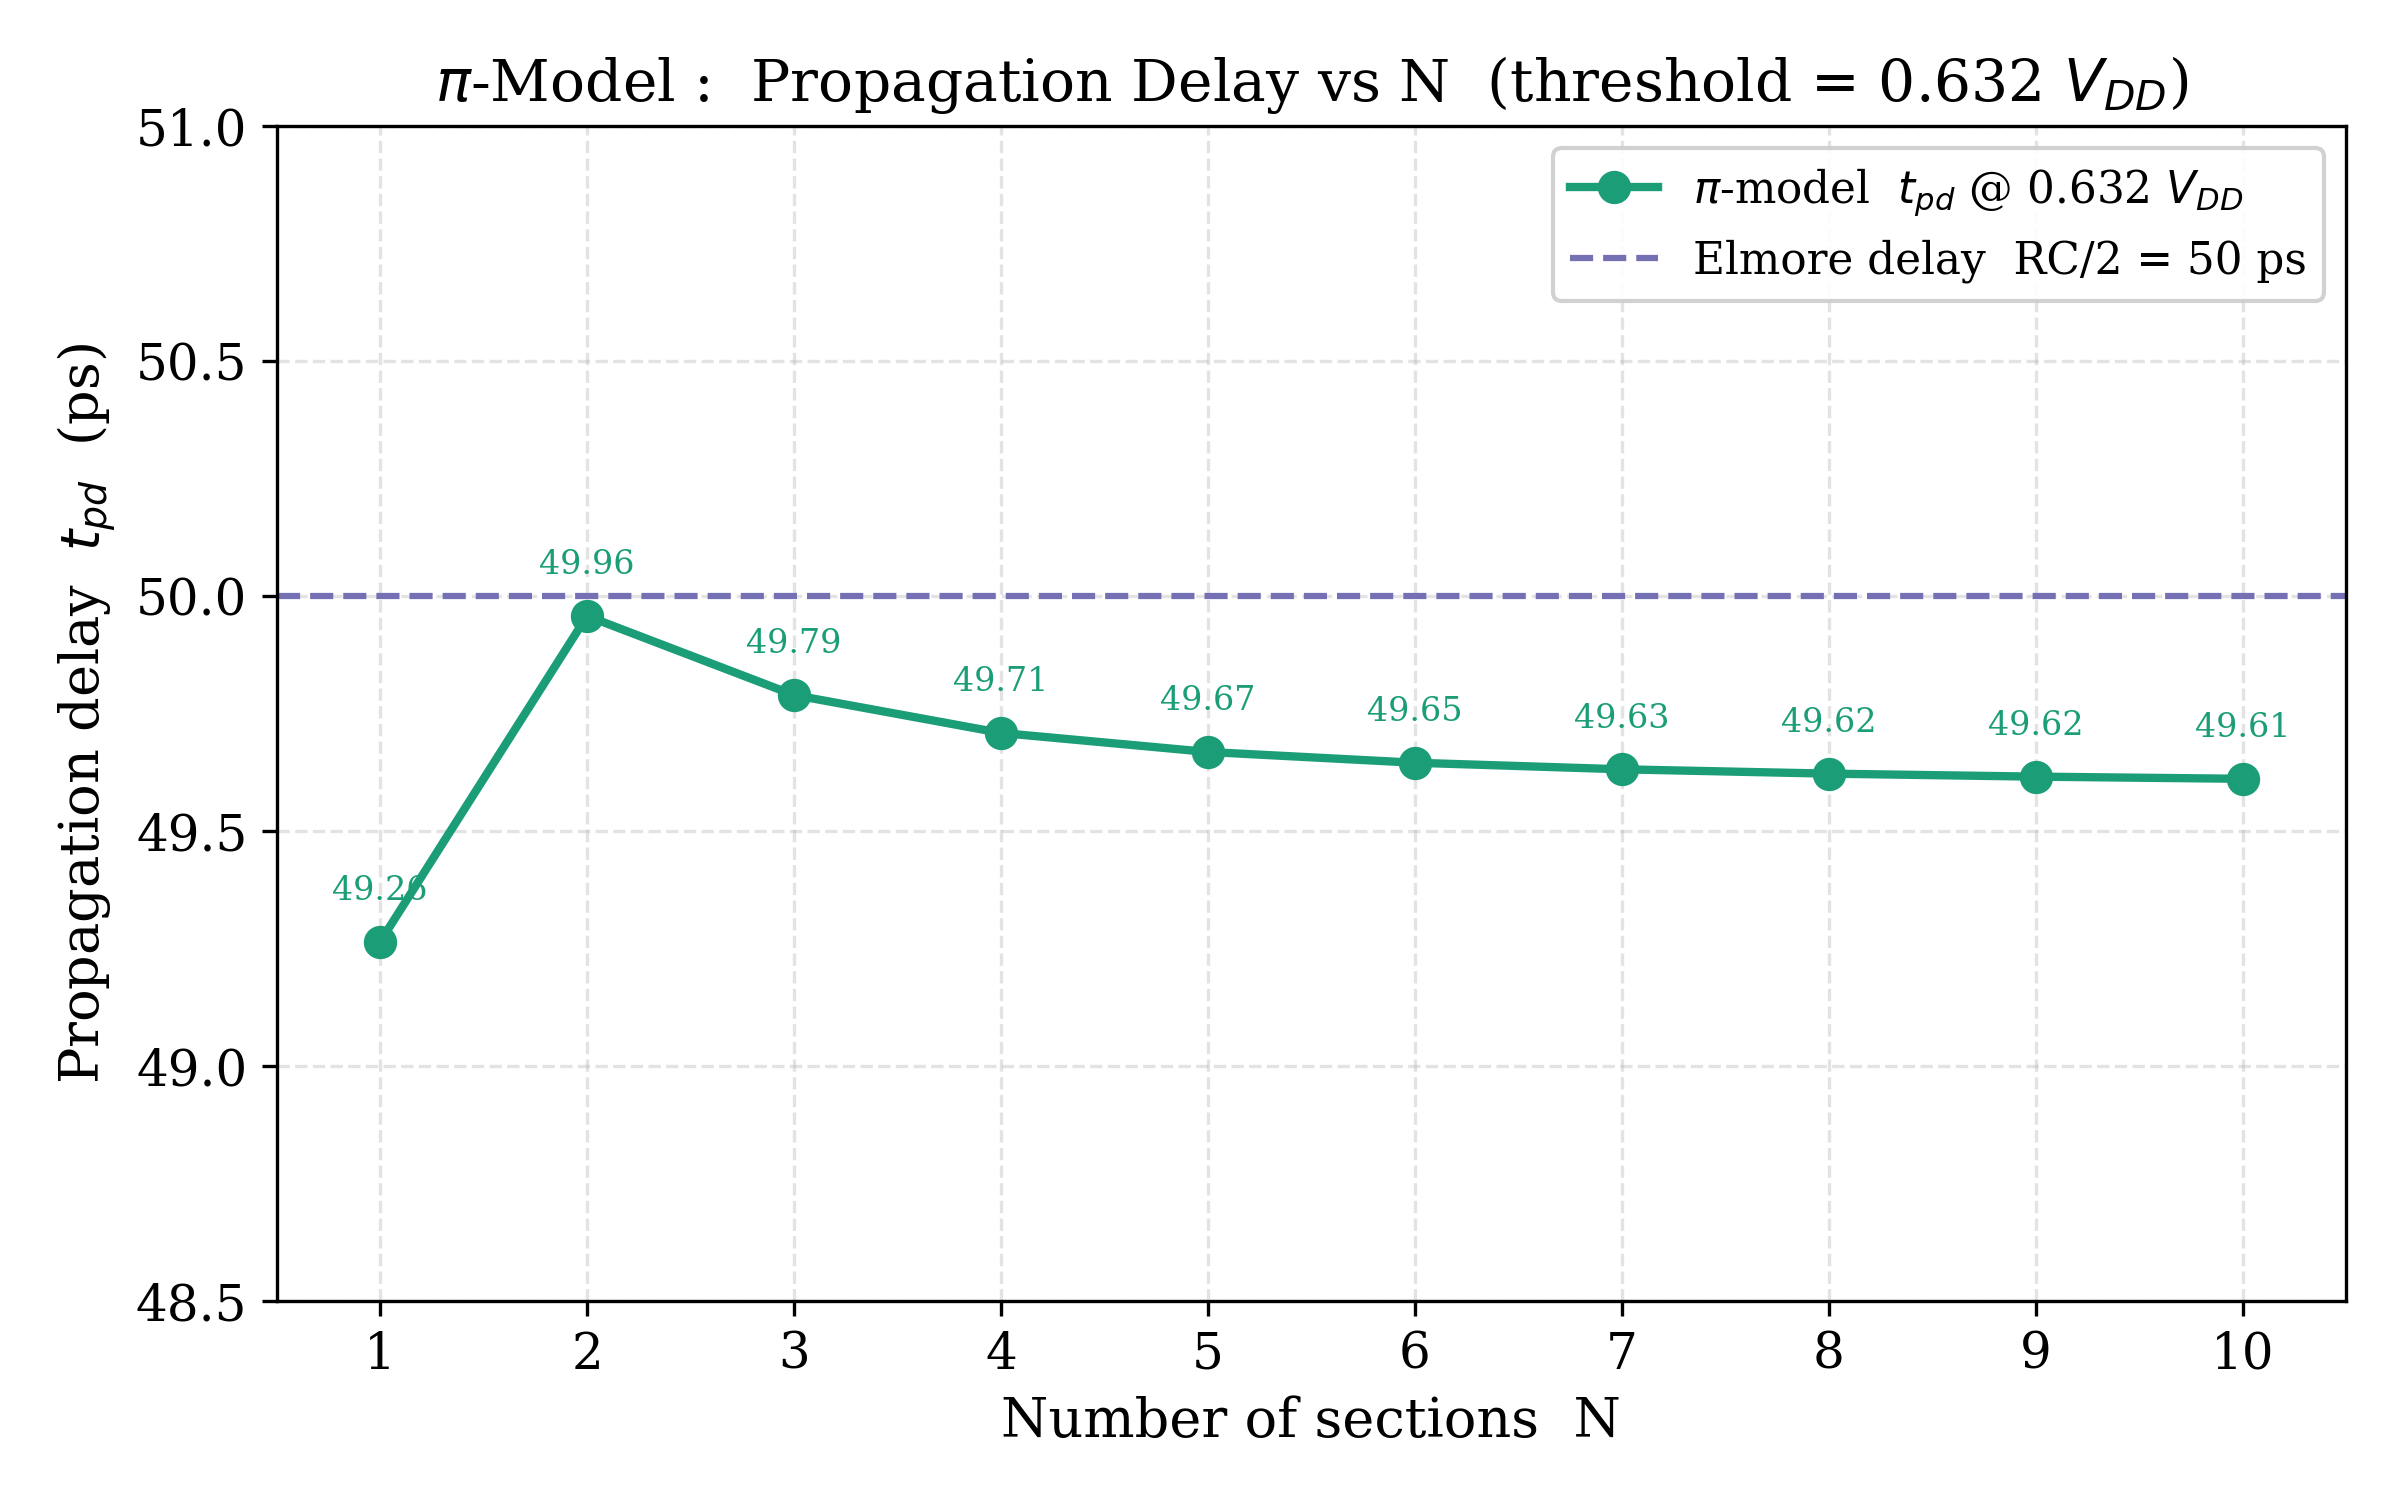
\includegraphics[width=6.1cm]{pi_topology/images/pi_tpd_vs_N_632VDD.png}\\[0.1cm]
    \scriptsize \textcolor{black!70}{Left: 0.5 $V_{DD}$ threshold \quad Right: 0.632 $V_{DD}$ threshold \quad (Fast edge $t_r = 5.65$\,ps)}
}
\hfill
\slidebox{6}{
    \centering
    \textbf{T-Topology: Propagation Delay vs N}\\[0.15cm]
    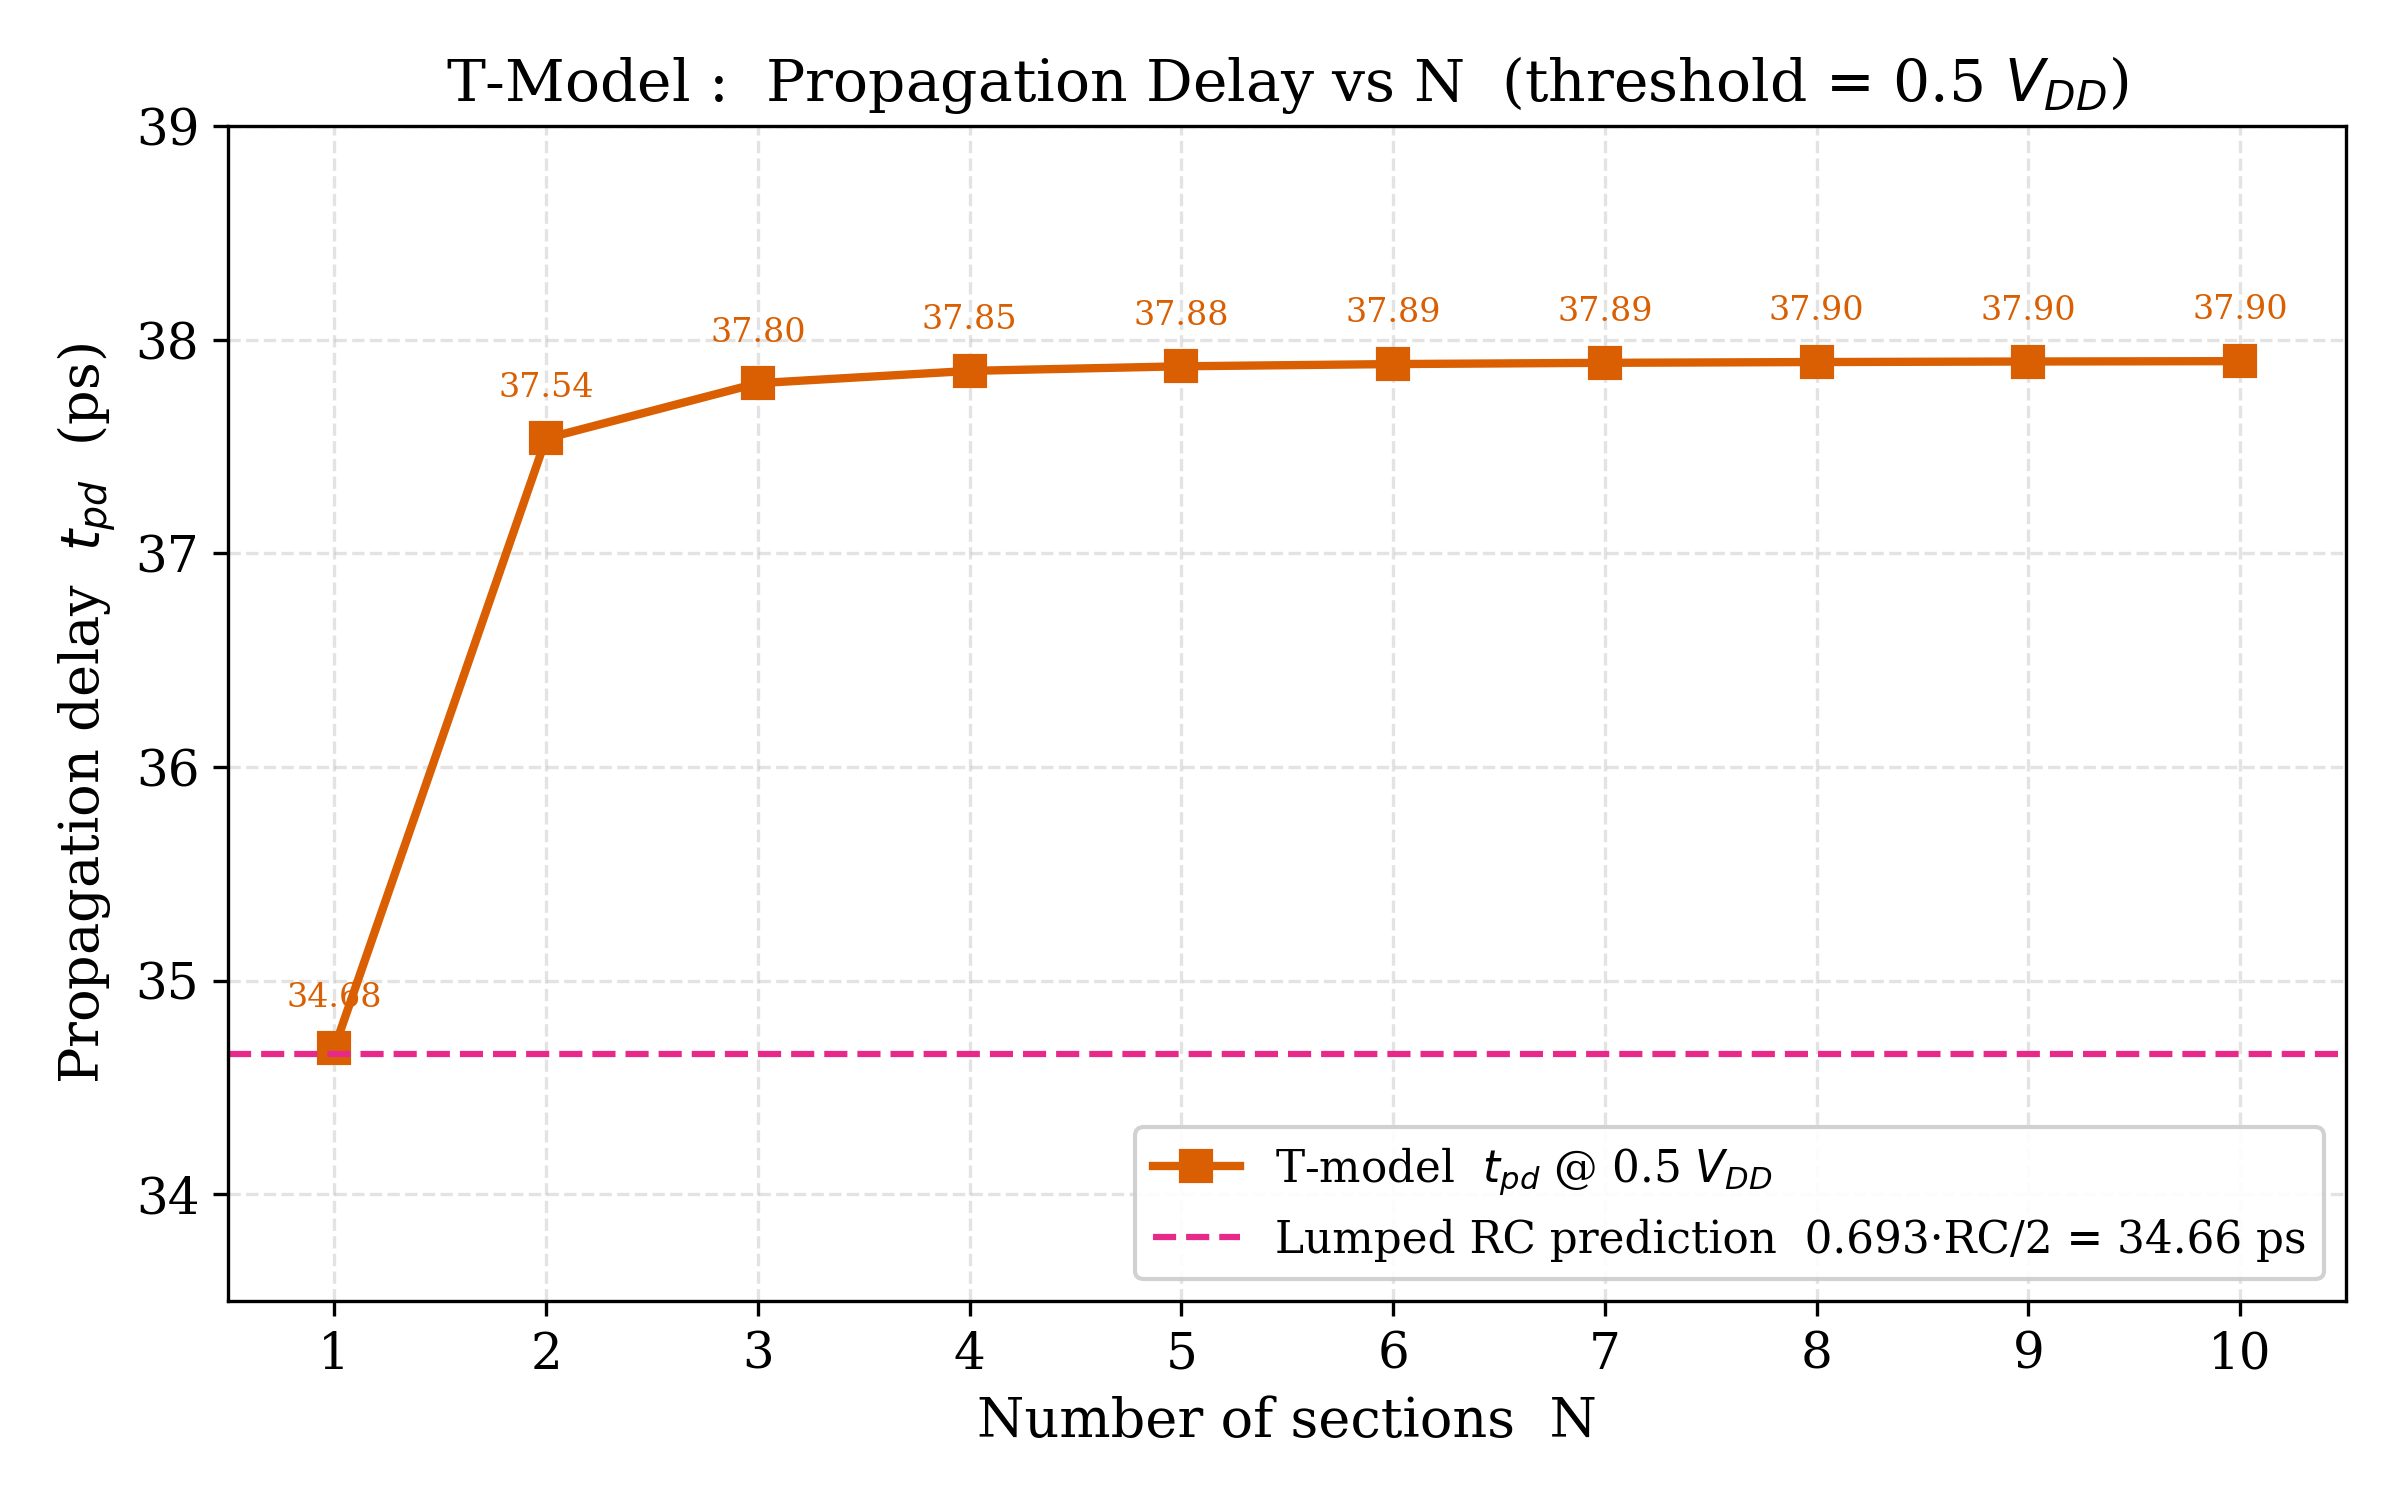
\includegraphics[width=6.1cm]{T_topology/images/T_tpd_vs_N_50VDD.png}\hfill
    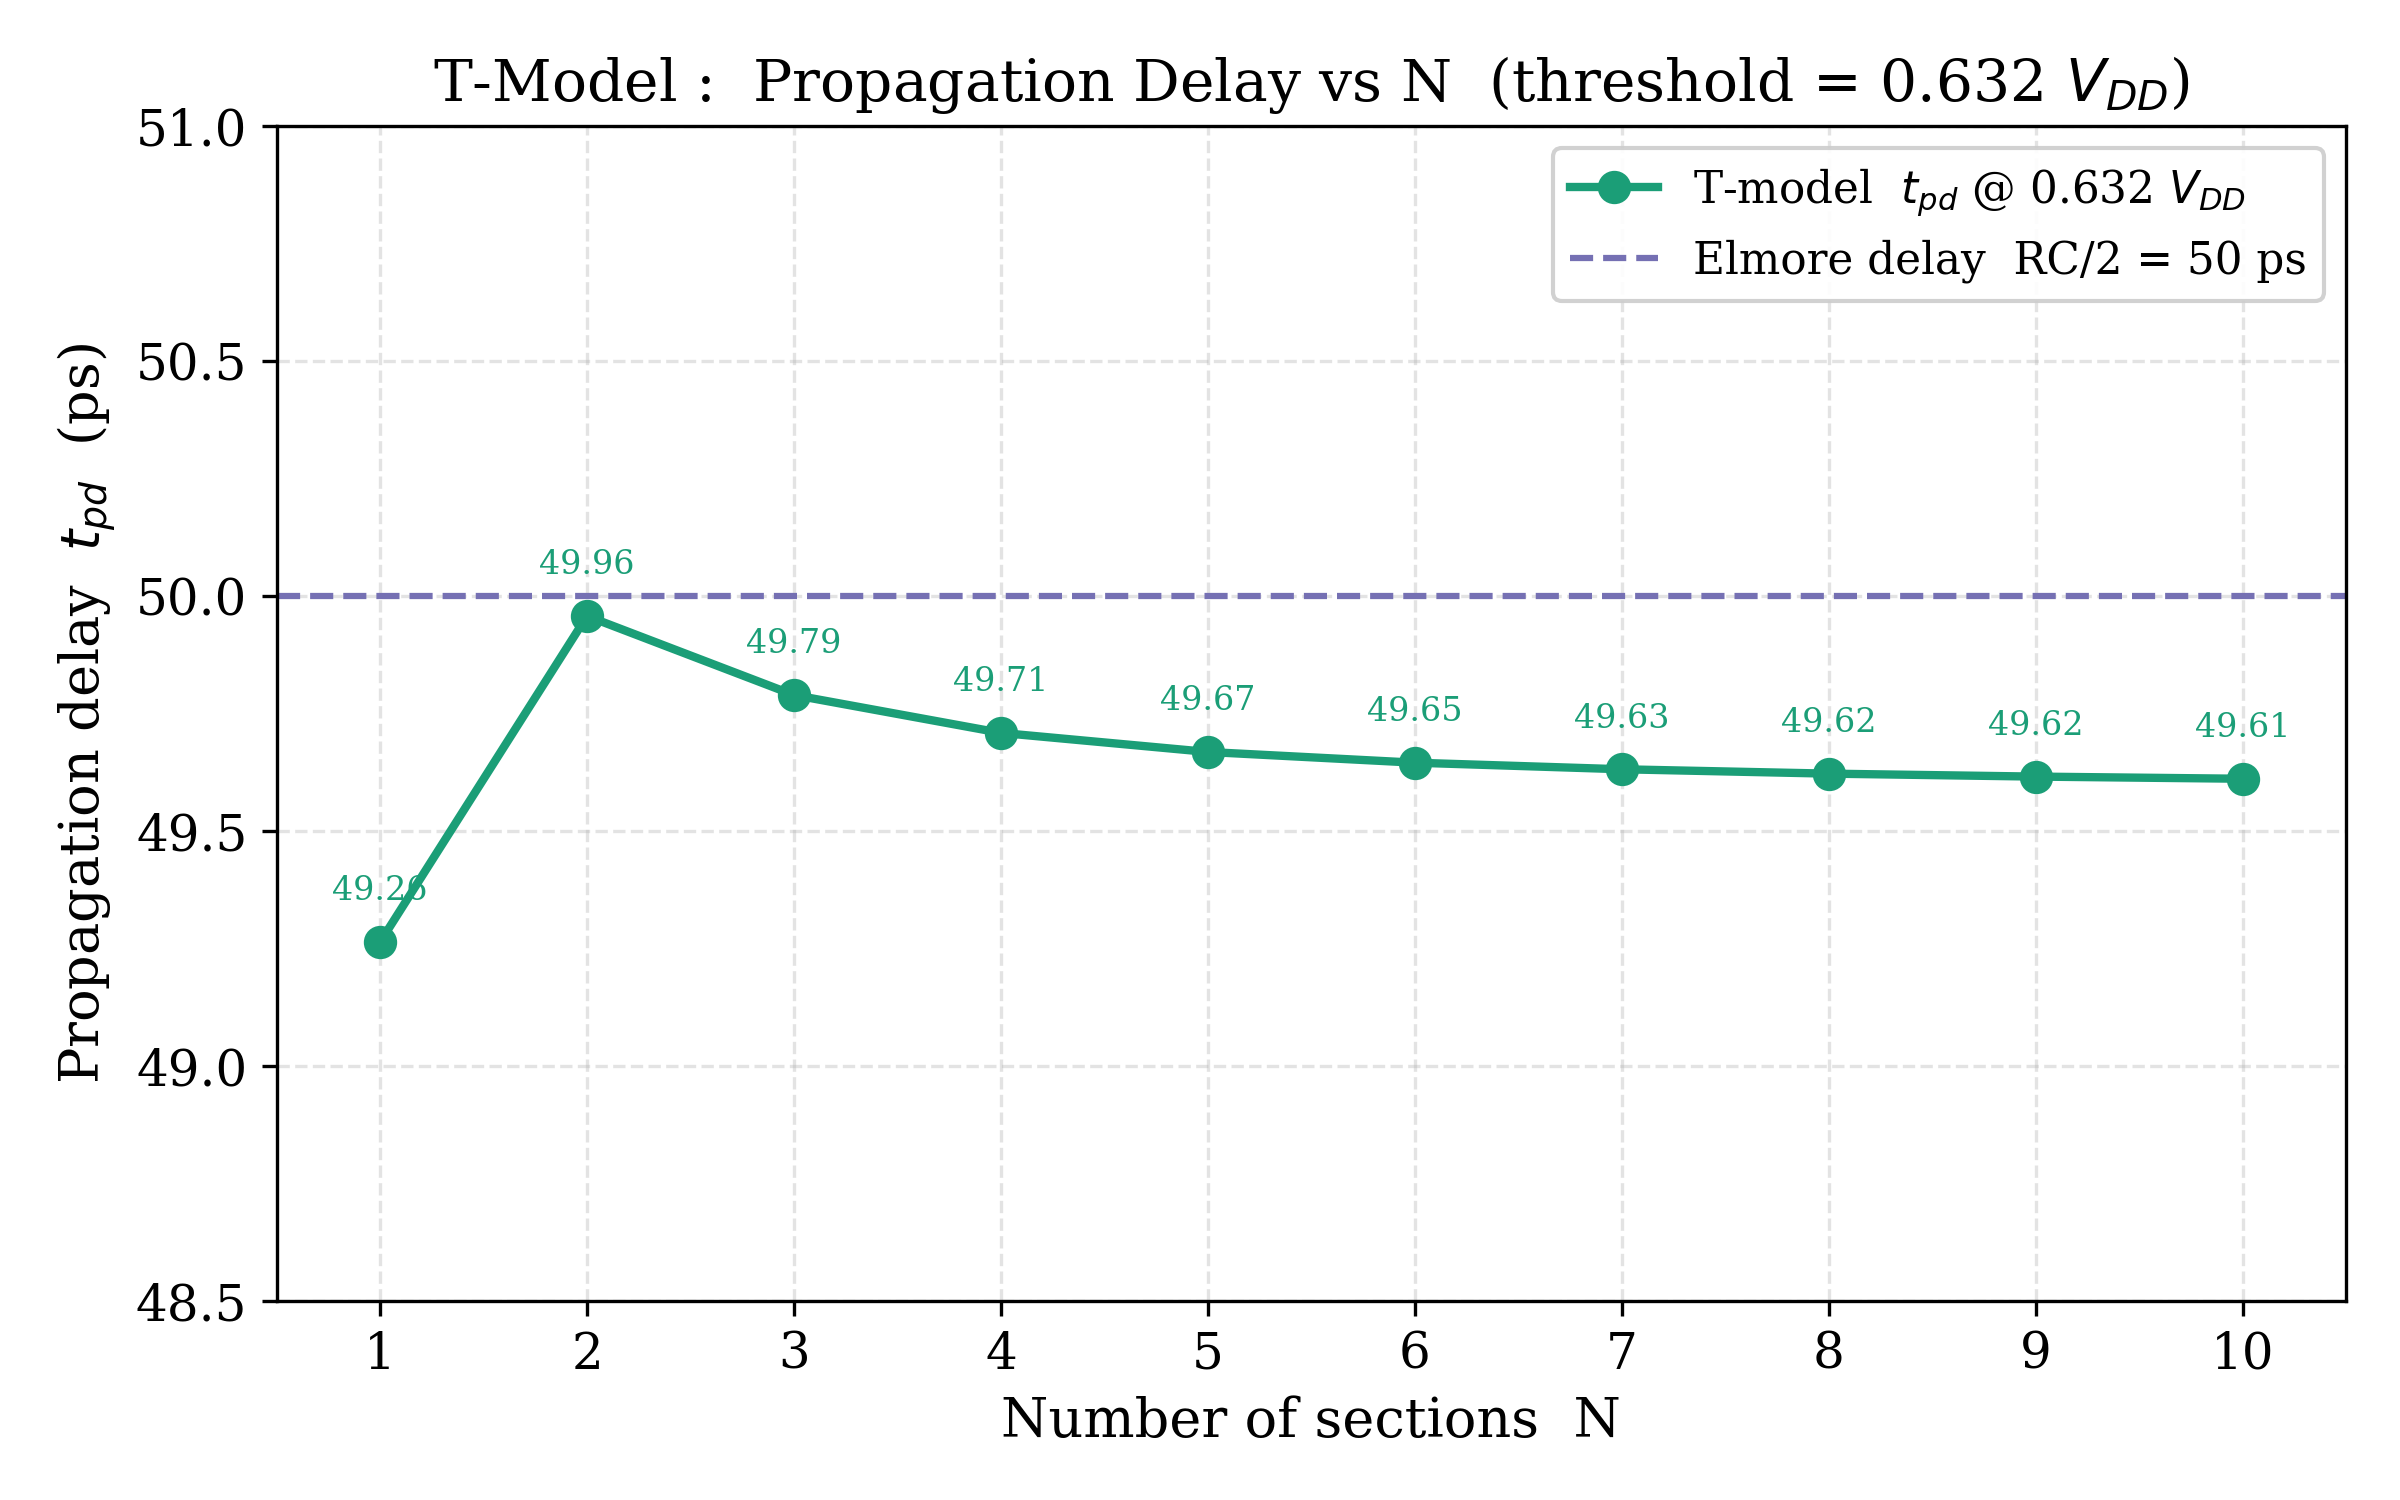
\includegraphics[width=6.1cm]{T_topology/images/T_tpd_vs_N_632VDD.png}\\[0.1cm]
    \scriptsize \textcolor{black!70}{Left: 0.5 $V_{DD}$ threshold \quad Right: 0.632 $V_{DD}$ threshold \quad (Fast edge $t_r = 5.65$\,ps)}
}

\vspace{0.7cm}

\noindent
\slidebox{7}{
    \centering
    \textbf{Slow-Edge Regime ($t_r = 400$\,ps)}\\[0.15cm]
    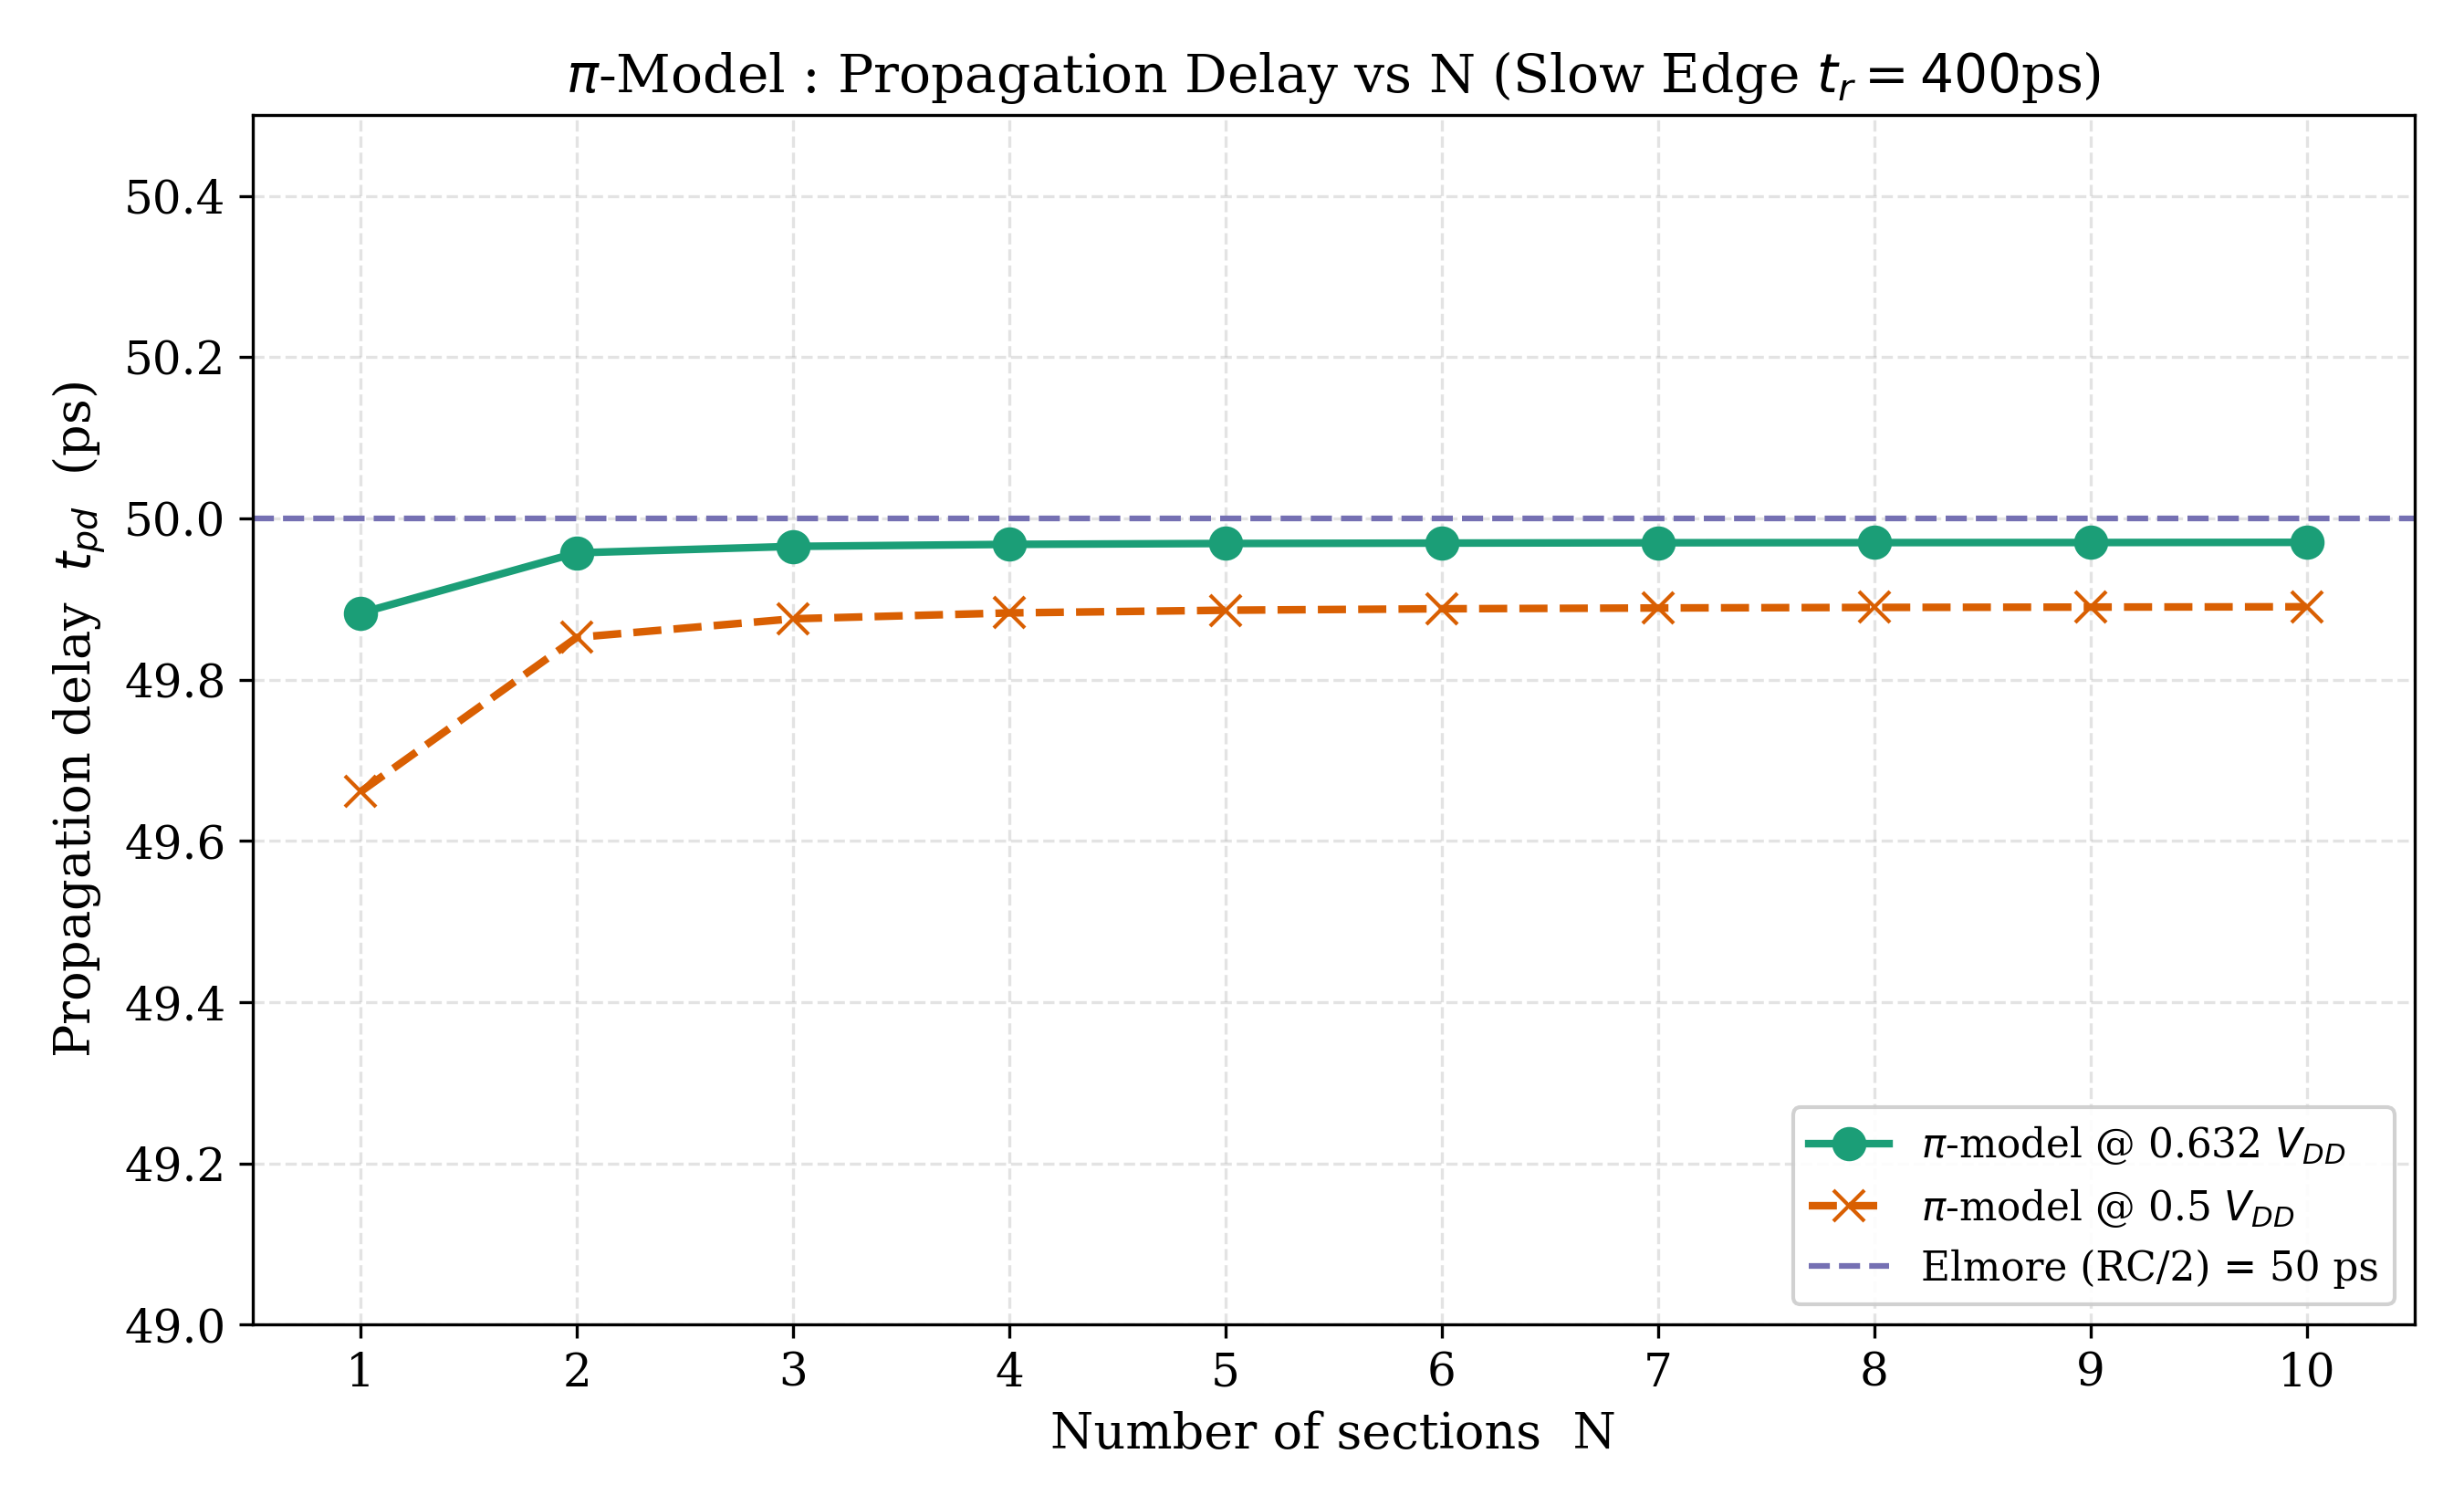
\includegraphics[width=6.1cm]{slower_edge_rate/images/pi_tpd_vs_N_slow_edge.png}\hfill
    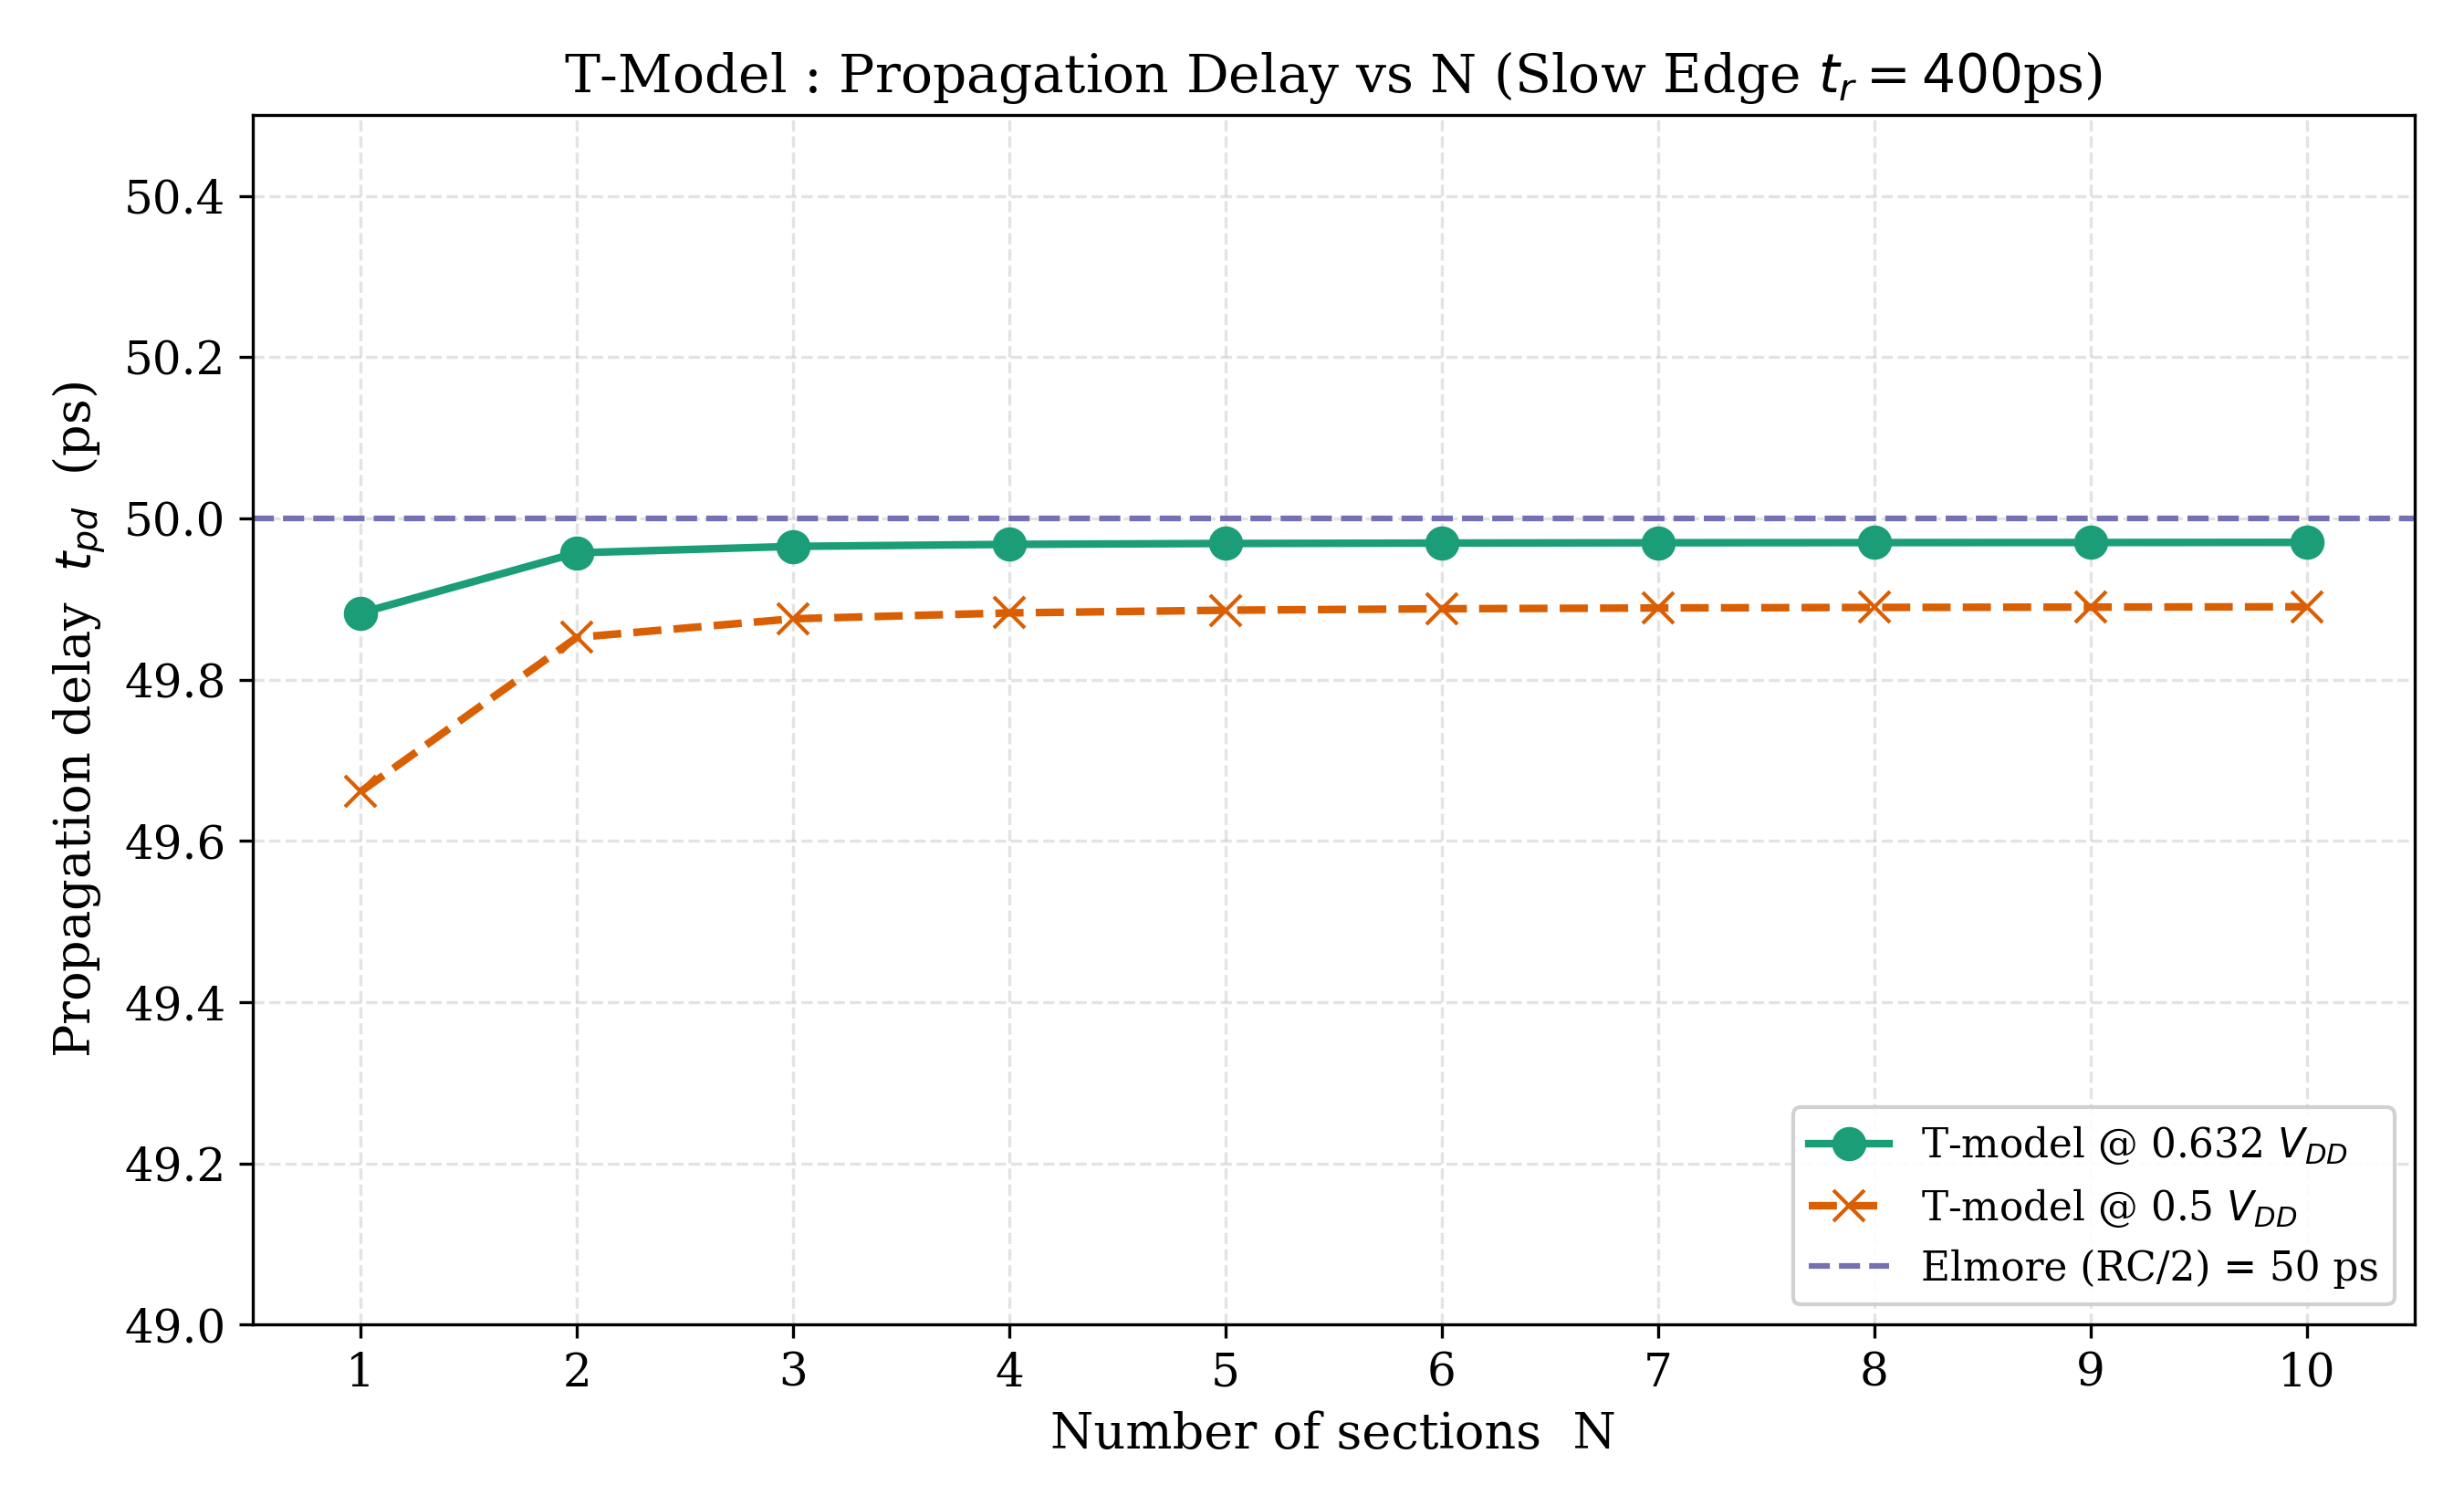
\includegraphics[width=6.1cm]{slower_edge_rate/images/T_tpd_vs_N_slow_edge.png}\\[0.1cm]
    \scriptsize \textcolor{black!70}{Left: $\pi$-model \quad Right: T-model. Delay approaches Elmore delay (50\,ps) regardless of threshold.}
}
\hfill
\slidebox{8}{
    \centering
    \textbf{Transient Step Response (Fast Edge)}\\[0.15cm]
    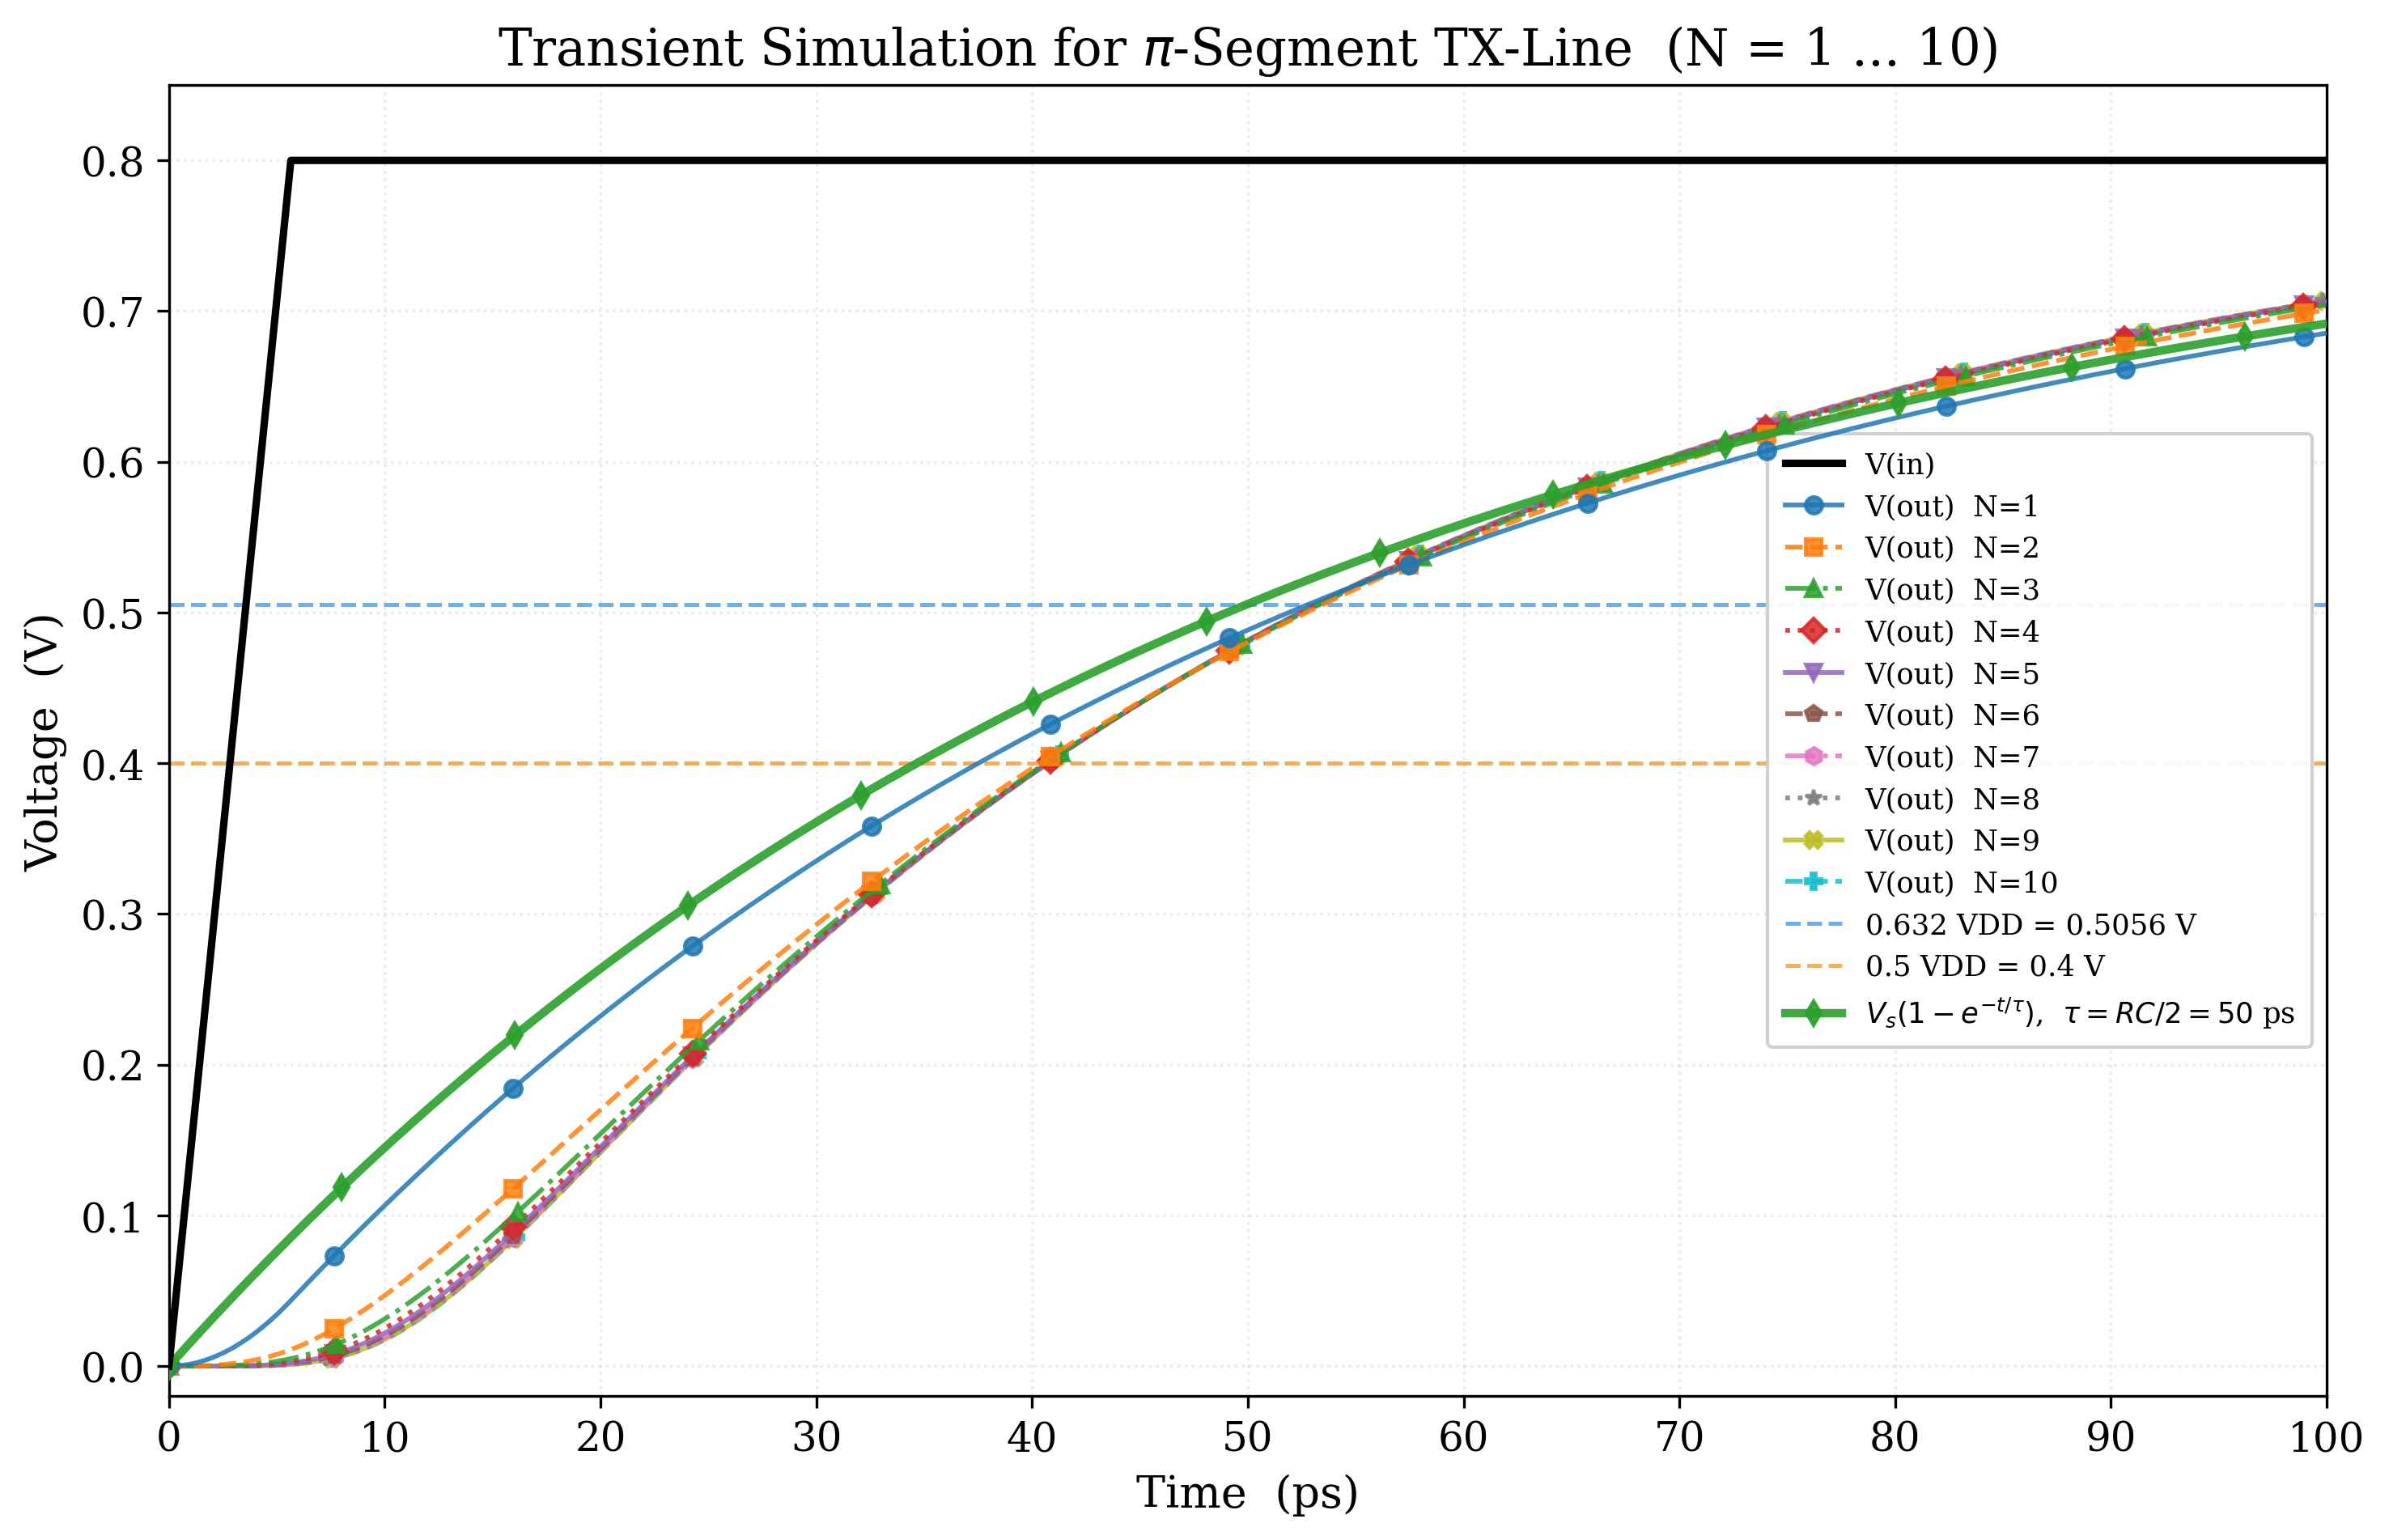
\includegraphics[width=6.1cm]{pi_topology/images/pi_transient_vin_vout_N1_to_N10.png}\hfill
    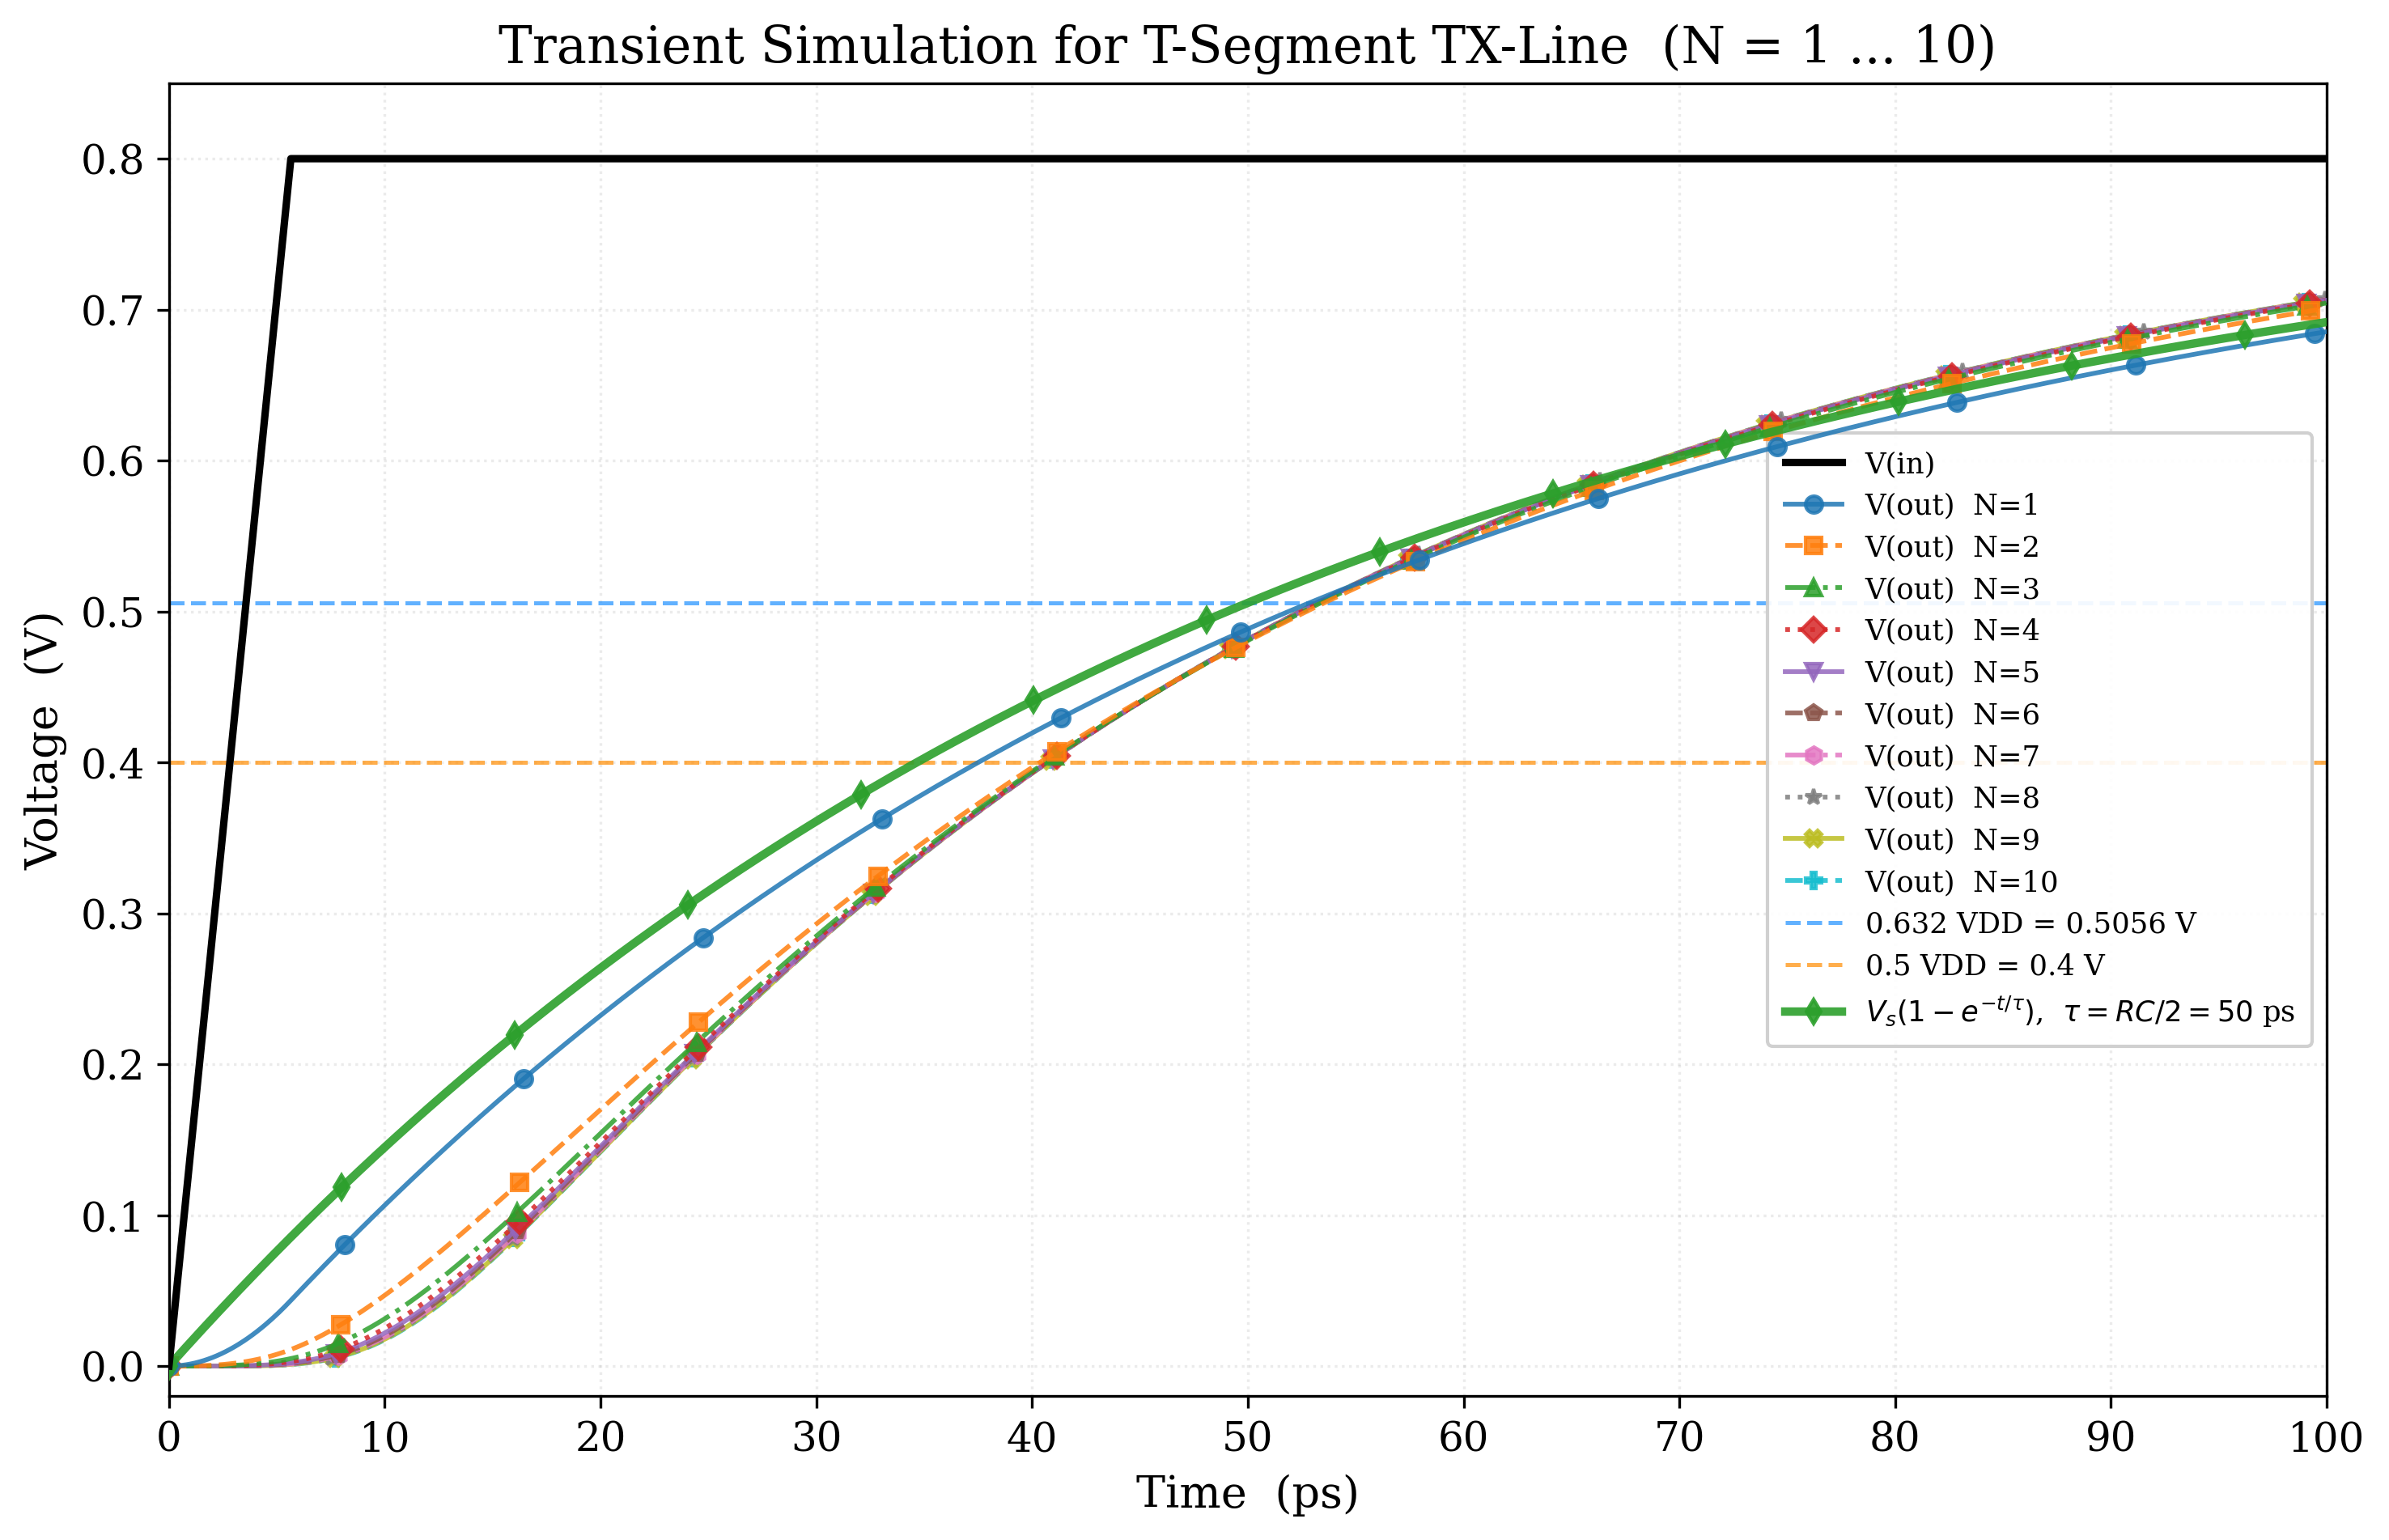
\includegraphics[width=6.1cm]{T_topology/images/T_transient_vin_vout_N1_to_N10.png}\\[0.1cm]
    \scriptsize \textcolor{black!70}{Left: $\pi$-model \quad Right: T-model. As $N \to 10$, response converges to distributed RC behavior.}
}

\end{document}
